\documentclass[11pt]{article}

\usepackage{array}
\usepackage{caption}
\usepackage{fancyhdr}
\usepackage[a4paper, margin=1in]{geometry}
\usepackage[final]{graphicx}
\usepackage[hidelinks, implicit=false]{hyperref}
\usepackage[newfloat]{minted}
\usepackage{xcolor}
\usepackage{subcaption}
\usepackage{listings,cleveref}
\usepackage{multimedia}
% \graphicspath{{./figures/}}

\definecolor{LightGray}{gray}{0.9}


% \newenvironment{code}{\captionsetup{type=listing}}{}
% \SetupFloatingEnvironment{listing}{name=Source Code}


\begin{document}
    \pagestyle{fancy}
    \setlength{\headheight}{13.6pt}

    \begin{titlepage}
        \begin{center}
            \vspace*{1cm}
            \Huge
            \textbf{Computer Science NEA 2025} \\
            \vspace*{2cm}
            \LARGE
            \textbf{Nathan Tatkowski}

            \vfill
            \includegraphics*[width=0.4\textwidth]{figures/igsLogo.jpg} \\
            \Large
            Invicta Grammar School \\
            Centre Number: \\
            Candidate Number: 
        \end{center}
    \end{titlepage}

    \tableofcontents
    \pagebreak
    \fancyhead[L]{Nathan Tatkowski}


    \section{Analysis}
        \subsection{Problem Identification}
            Often times during research it is important and very helpful to be able to visualise the events that are being analysed. When working with models in two dimensions, it is easy enough to be able to draw out an accurate diagram, even if it may be tedious. However, 2D models are nowhere near as applicable or useful as considering events in three dimensions, stemming from the fact that the world we live in is three-dimensional. Something that would aid intuition and help in problem-solving would be a way to have events modelled quickly, accurately, and clearly, given a set of initial conditions.

        \subsection{Identification of why this problem is solvable by computational methods}
            The key requirements stated above (accuracy, haste, and clarity) lend themselves very well to using computational methods. Computers are able to make calculations orders of magnitude faster than by hand or by analogue machine, and to a virtually arbitrary degree of accuracy. Many modern central processing units (CPUs) are also able capable of making use of concurrent processing, further increasing the advantage that a computer would have over a human. Graphical processing units (GPUs) are specifically designed for parallel processing, making them especially useful for graphics, which would allow for high quality renders for the user to be able to see. Any data that you would need to consider can be displayed in a clear and user-friendly fashion, making it highly customisable to fit the individual persons needs and for many attributes to be studied at the same time.

        \subsection{Description of the Current System}
            Without using computer simulations, the usual process is to produce a handful of equations by hand that would model the attributes of an object, commonly the path it takes in three-dimensional space. This has the benefit of giving exact values and equations that are very useful when trying to understand the underlying reasons for an event happening. For example when considering a pendulum, it is clear from the equation $$ T = 2 \pi \sqrt{\frac{L}{g}} $$ that the period of the pendulum $T$ does not depend on the mass of the object doing the swinging. However, when running computer simulations, such relationships may not be as obvious, and as computers aren't able to analytically solve problems (i.e. through the use of rigorous mathematics), this is a drawback that I will have to consider.
            
        \subsection{Identification of Stakeholders}
            After considering the problem I identified the following groups that could use a solution to this problem, as well as having useful insight on how a program like this should function.
            \begin{itemize}
                \item \textbf{University Students} often have to deal with complex systems and a way of visualising them would be very beneficial. I have been able to contact a student at the University of Aberdeen doing a masters in electrical and mechanical engineering. Their name is Hugo, and they are 21-years-old.
                \item \textbf{A-Level Students}, specifically students taking physics,  would be able to greatly further their understanding of core concepts and be able to explore new ideas on their own. I have been able to communicate with Daniel, a year 12 physics student, about being a stakeholder for this project.
                \item \textbf{Teachers} of A-Level and below could make great use of simulation software in order to make learning much easier with models and demonstrations that are clear and easy to understand. I have been able to contact Mr Waters about being a stakeholder for this project, who teaches physics at Invicta Grammar School.
            \end{itemize}
            
        \subsection{Identification of User Needs and Acceptable Limitations}
            Summary of key take aways from interviews:
            \begin{itemize}
                \item My stakeholders are people who generally enjoy doing physics and find it enjoyable, although they all acknowledge how much work it can be. As such, decreasing workload without completely eliminating need for human input would be important, as that would make it less enjoyable.
                \item People struggle with abstract concepts, and a common topic seems to be electricity and electricals systems, as well as visualising some key concepts in physics such as waves. Considering a way to visualise circuits and the physics going on in those would be useful all of my stakeholders.
                \item Two out of three of my stakeholders said that they enjoyed astrophysics, so considering some sort of astro-mechanics simulation could be of use to them, as visualising large bodies moving in space is difficult.
                \item People find graphs very useful in visualisation and aiding intuition. Some sort of real-time graphing of attributes could be something useful to consider in the final product.
                \item All my stakeholders are competent in using simulation software, or don't mind spending time to learn how to use one properly. This would mean that accuracy and functionality could be prioritised over general user experience if necessary. 
            \end{itemize}

        \subsection{Existing Solutions}
            \subsubsection{Analytic Methods}
                Analytic methods are very common as they require little cost or set-up and their effectiveness only depends on how well you understand the physics that you are doing. Since my stakeholders enjoy doing physics and are also quite good at it, they are all well versed in spending time going through calculations in order to achieve a set of mathematical equations that describe the system being modelled. 

                \begin{figure}[!ht]
                    \begin{center}
                        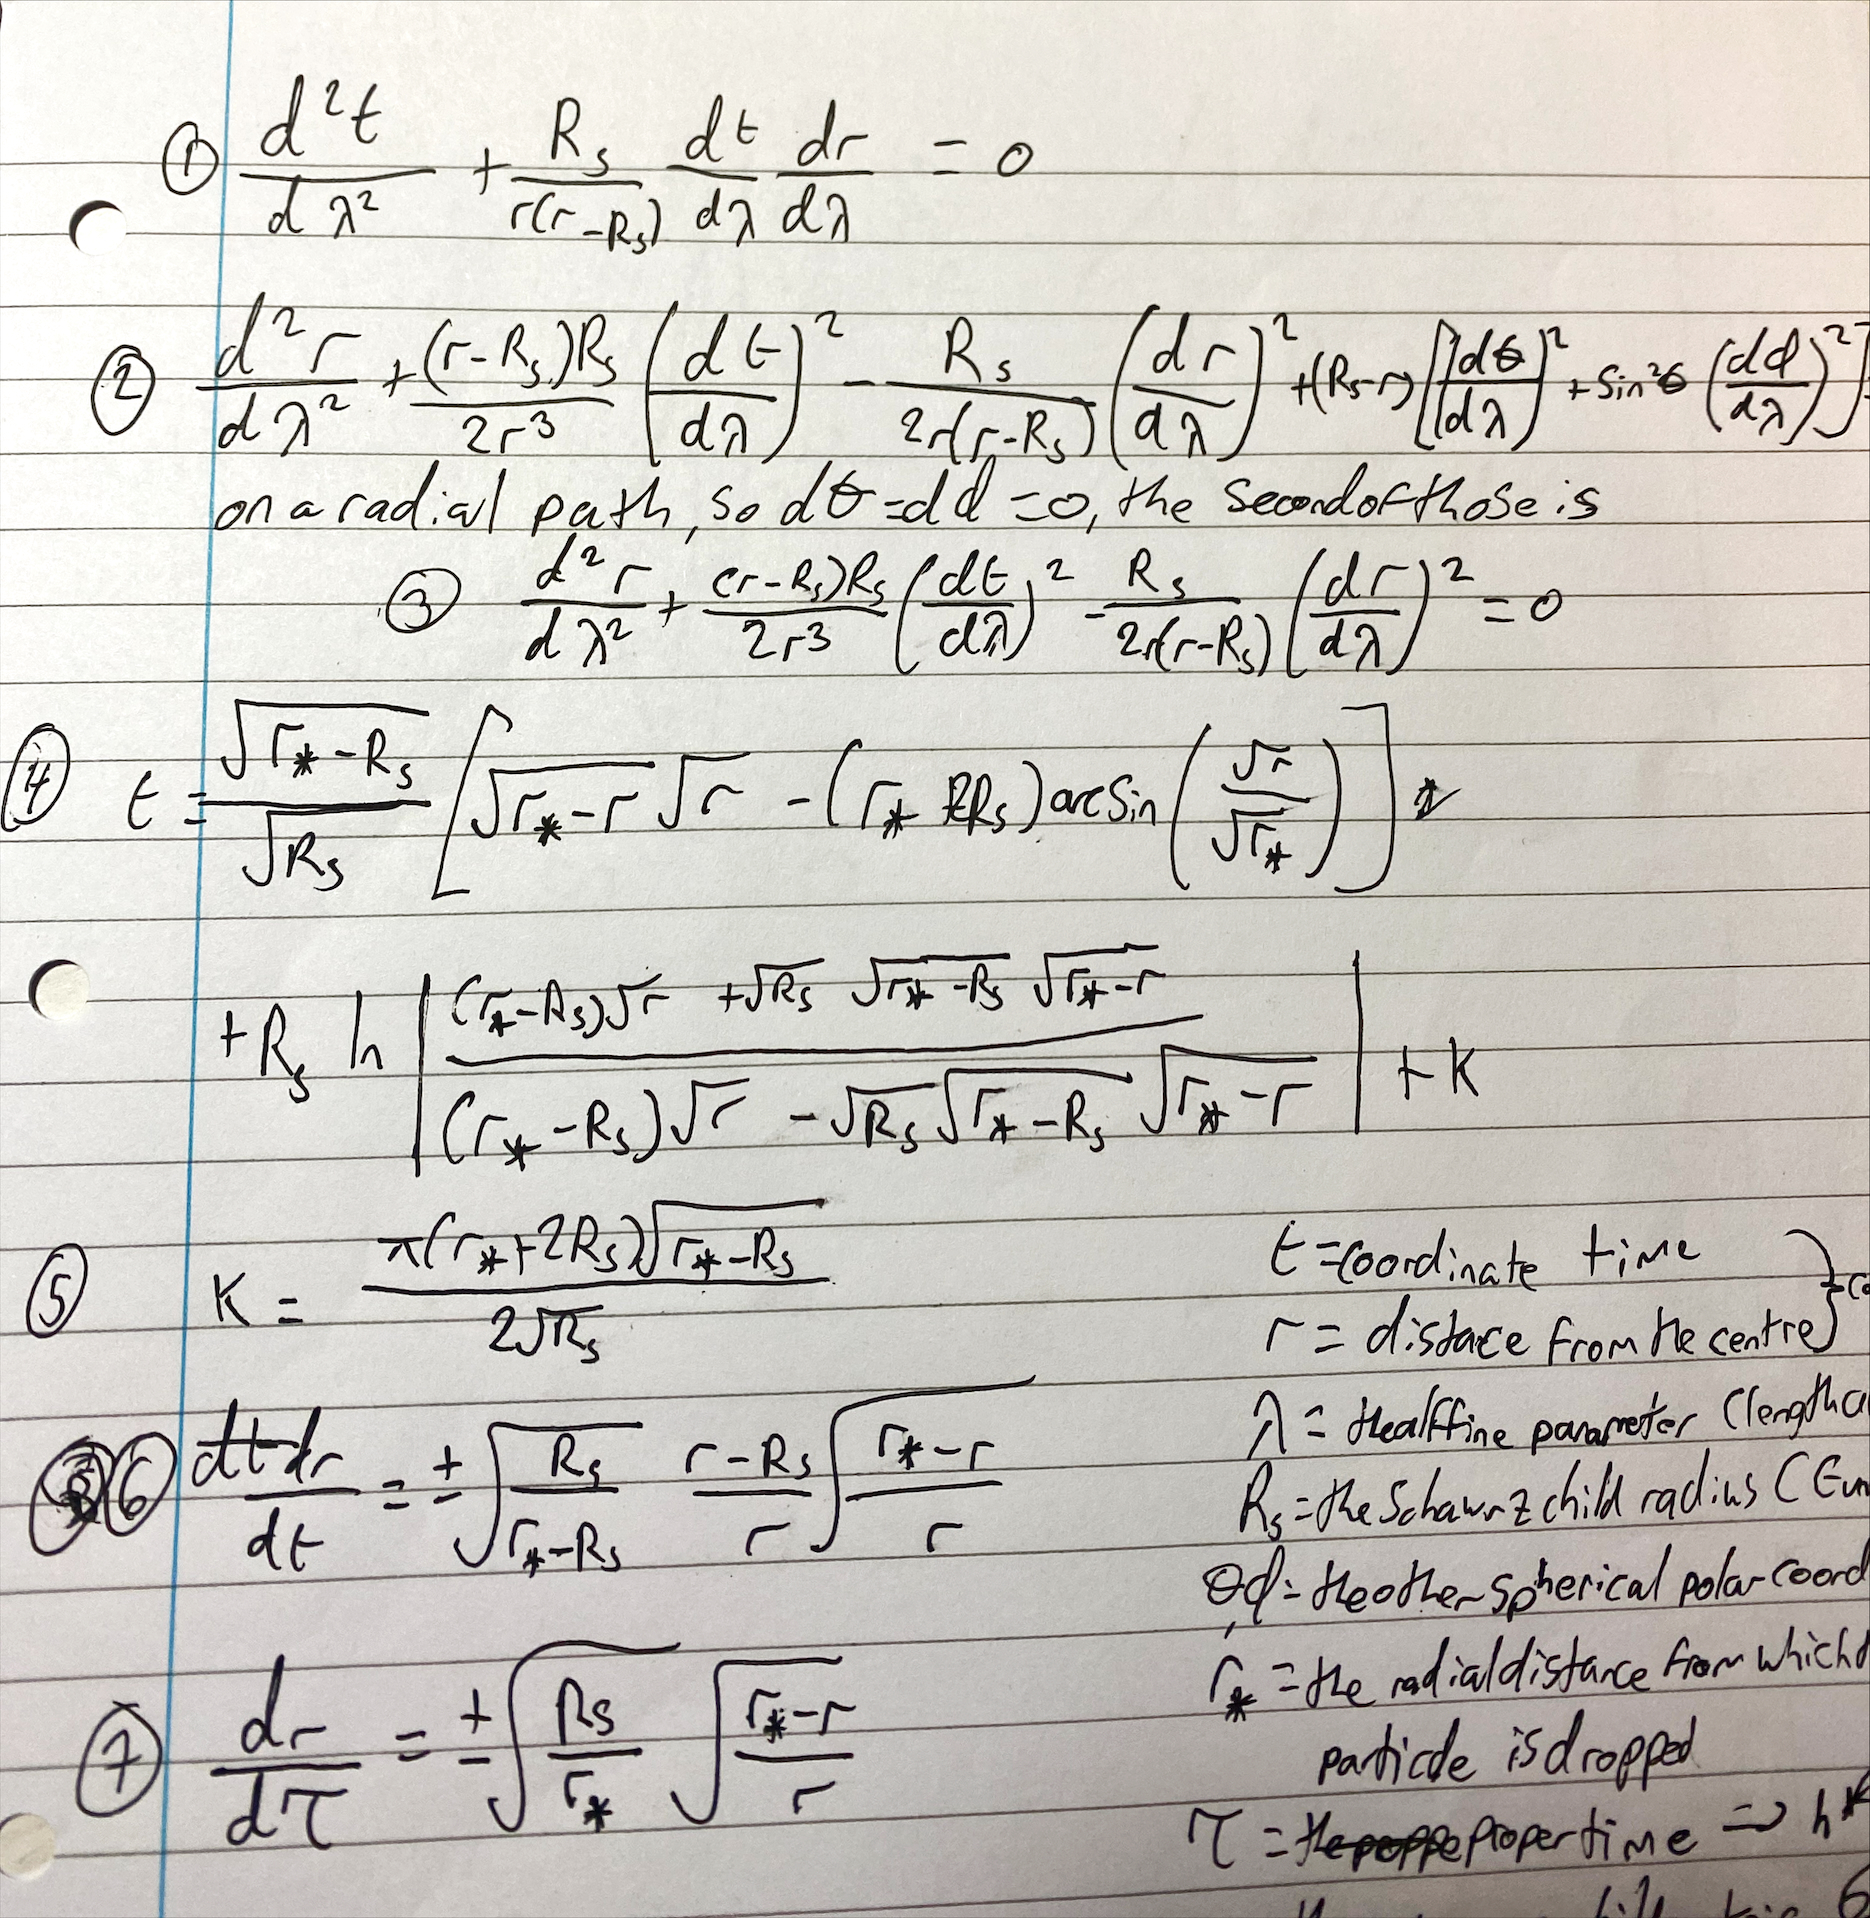
\includegraphics[width=0.3\textwidth]{figures/daniel_working.jpeg}
                    \end{center}
                    \caption{A sample of Daniel's working out}
                    \label{fig:daniel_working}
                \end{figure}

                As seen in Figure~\ref{fig:daniel_working}, one clear disadvantage of working on paper is how messy and disorganised it can get. It can quickly become difficult to read and follow if you don't take enough care with your presentation, which would hinder understanding of the system being studied, and a piece of computer software would be better in this aspect due to its consistency. However, the flexibility of working on paper and being able to freely annotate and draw diagrams would be very difficult, if not impossible, to emulate on a computer. 

                Another disadvantage of analytic methods is that not all systems are solvable through analytic methods, depending on how simple or complex you decide to make your model. For example, if considering the free fall of an object, a simple model would only consider the effects of gravity, whereas a more complex would take into account the initial altitude, effects of air resistance, and changes in air pressure. Obviously the former is much easier to work through, but it is also not immediately obvious that the latter isn't actually solvable analytically, and numerical methods have to be used. Since a computer could only approach a problem numerically, that would mean computer software would have a greater range of problems that it could tackle, at the cost of accuracy (which can be made negligible) and of course the enjoyment of doing the work yourself.

            \subsubsection{Desmos}
                \begin{figure}[!ht]
                    \begin{center}
                        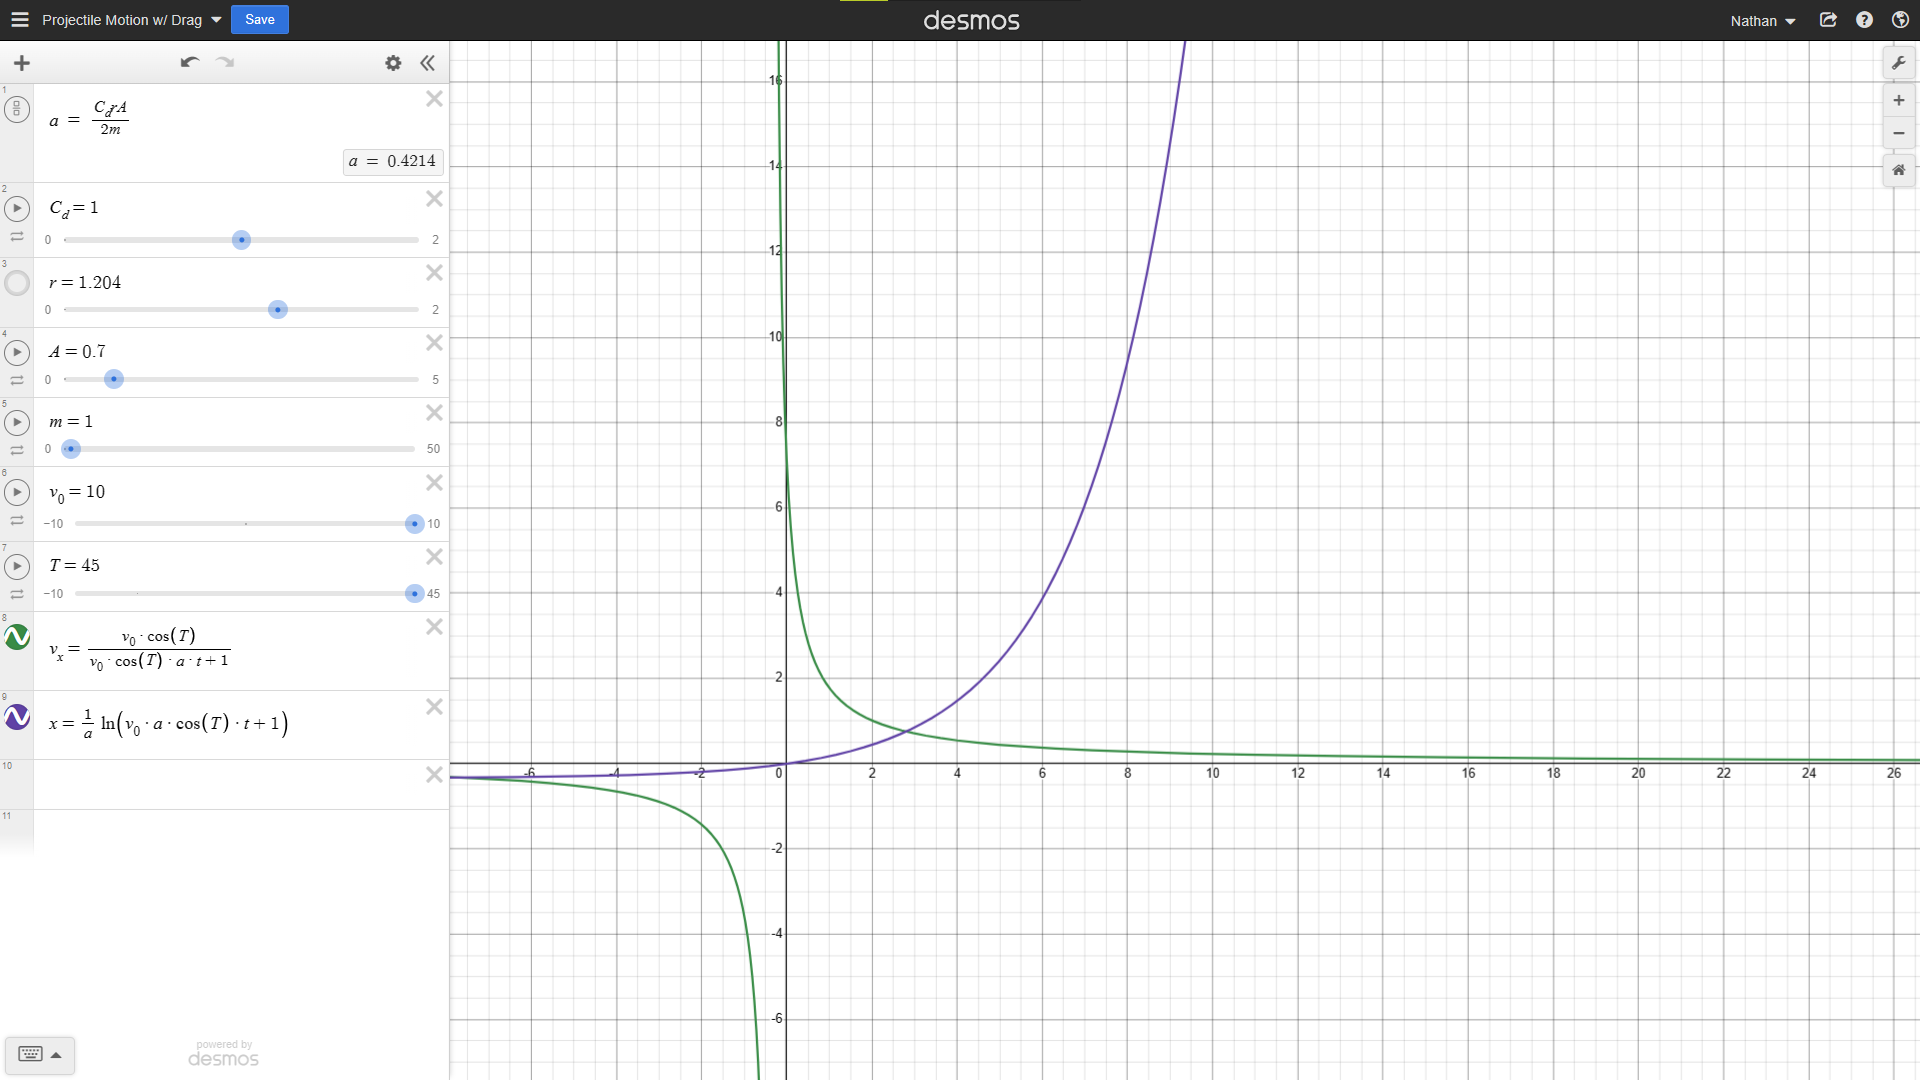
\includegraphics[width=.5\textwidth]{figures/desmos.png}
                    \end{center}
                    \caption{Desmos graphing software}
                    \label{fig:desmos}
                \end{figure}

                In Figure~\ref{fig:desmos} above, Desmos has been used in order to see how attributes of an object change (specifically the $x$ position and velocity with respect to time of an object experiencing drag). Desmos is great in order to aid intuition and view general trends, however you still need to work through equations in order to have something to graph, and Desmos won't give exact values for solutions, but the final visualisations are still very useful. 

                The simplicity of Desmos allows it to be very versatile, but that also means its more of a jack-of-all-trades and master of none, so it wouldn't be very good for a more specialised application (like the ones being considered).



            \subsubsection{Kerbal Space Program}
                Kerbal Space Program here

        \subsection{Success Criteria of the Proposed System}
        \subsection{Data Source(s)}
        \subsection{Volumetrics - Data Volumes}
        \subsection{Analysis Data Dictionary}
        \subsection{Data Flow Diagrams for Existing and Proposed System}
        \subsection{Justification of Chosen Solution}
        \subsection{Hardware and Software}
        \subsection{Entity-Relationship Models}
        \subsection{Identification of Objects and Object Analysis Diagrams}

    \section{Design}
        \subsection{Overall System Design}
        \subsection{Description of Modular Structure of System}
        \subsection{Definition of Data Requirements}
        \subsection{Identification of Appropriate Storage Media}
        \subsection{Identification of Processes and Suitable Algorithms for Data Transformation and Completion of the Solution}
        \subsection{Sample of Algorithms}
        \subsection{User Interface Design Rationale and Usability Features}
        \subsection{Security and Integrity of Data}
        \subsection{System Security (Access Control)}
        \subsection{Overall Test Strategy}

    \section{Implementation}
        \subsection{Annotated Listing of the Program(s)}
        \subsection{Annotated "Design Views" showing details of application-generated forms, reports, queries, buttons, cross tabulations, etc.}
        \subsection{Procedure and Variable List}
        \subsection{Testing to inform development - Testing at each stage}
        \subsection{Re-Testing}

    % Join with previous section 
    \section{Testing}
        \subsection{Test Plan}
        \subsection{Test Data}
        \subsection{Areas to Test}
        \subsection{Tables}
        \subsection{Justification of Data Selection}
        \subsection{Evidence of Testing}
        \subsection{Program Listing}
    
    \section{Evaluation}
        \subsection{Comparison of Performance of your System against Success Criteria}
        \subsection{Analysis of User Feedback}
        \subsection{Evaluation of Usability Features}
        \subsection{Maintenance Issues and Limitations of the Product}
        \subsection{Improvements and Possible Extensions}
        

\end{document}